\documentclass[11pt,a4paper]{article}
\usepackage[utf8]{inputenc}
\usepackage[T1]{fontenc}
\usepackage{geometry}
\usepackage{graphicx}
\usepackage{xcolor}
\usepackage{tcolorbox}
\usepackage{booktabs}
\usepackage{amsmath}
\usepackage{amssymb}
\usepackage{hyperref}
\usepackage{fancyhdr}
\usepackage{listings}
\usepackage{tikz}
\usepackage{enumitem}

\geometry{margin=1in}

% Define colors
\definecolor{primarycolor}{RGB}{66, 133, 244}
\definecolor{secondarycolor}{RGB}{52, 168, 83}
\definecolor{accentcolor}{RGB}{251, 188, 5}
\definecolor{darkgray}{RGB}{66, 66, 66}
\definecolor{lightgray}{RGB}{245, 245, 245}
\definecolor{codebackground}{RGB}{248, 249, 250}

% Configure hyperlinks
\hypersetup{
    colorlinks=true,
    linkcolor=primarycolor,
    urlcolor=primarycolor,
    citecolor=primarycolor
}

% Configure code listings
\lstset{
    backgroundcolor=\color{codebackground},
    basicstyle=\ttfamily\small,
    breaklines=true,
    frame=single,
    rulecolor=\color{lightgray},
    numbers=left,
    numberstyle=\tiny\color{darkgray},
    keywordstyle=\color{primarycolor}\bfseries,
    commentstyle=\color{secondarycolor}\itshape,
    stringstyle=\color{accentcolor}
}

% Header and footer
\pagestyle{fancy}
\fancyhf{}
\fancyhead[L]{\small Q-NarwhalKnight Mainnet}
\fancyhead[R]{\small Block Rewards \& Emission Schedule}
\fancyfoot[C]{\thepage}
\renewcommand{\headrulewidth}{0.4pt}

\title{
    \Huge\textbf{Q-NarwhalKnight Mainnet} \\
    \vspace{0.3cm}
    \Large Block Production \& Reward System \\
    \vspace{0.5cm}
    \large\textit{DAG-BFT Consensus + Time-Based Halving}
}

\author{
    \textbf{Q-NarwhalKnight Development Team} \\
    \texttt{https://quillon.xyz}
}

\date{\today}

\begin{document}

\maketitle

\begin{abstract}
This document provides comprehensive technical specifications for the Q-NarwhalKnight mainnet, detailing the dual-layer architecture: high-throughput DAG-BFT consensus producing 2-10 blocks per second, and a time-based reward halving system that occurs every 4 years (calendar-based, not block-based). The system implements Bitcoin-inspired economics with an initial reward of 0.05 QUG per block, halving every 4 years until reaching a maximum supply of 21 million QUG asymptotically over approximately 256 years.
\end{abstract}

\tableofcontents
\newpage

% ============================================================================
\section{Executive Summary}
% ============================================================================

\subsection{Quick Facts}

\begin{table}[h]
\centering
\begin{tabular}{ll}
\toprule
\textbf{Parameter} & \textbf{Value} \\
\midrule
\multicolumn{2}{c}{\textit{DAG-BFT Consensus Layer}} \\
\midrule
Block Production Rate & 2-10 blocks/second \\
Consensus Type & DAG-Knight + Narwhal \\
Byzantine Fault Tolerance & Asynchronous BFT \\
\midrule
\multicolumn{2}{c}{\textit{Mining Reward System}} \\
\midrule
Initial Block Reward & 0.05 QUG \\
Halving Method & \textbf{TIME-BASED (Calendar)} \\
Halving Interval & Every 4 years \\
Development Fee & 1\% (0.0.05 QUG initially) \\
Miner Reward & 99\% (49.0.05 QUG initially) \\
\midrule
\multicolumn{2}{c}{\textit{Economic Parameters}} \\
\midrule
Maximum Supply & 21,000,000 QUG \\
Genesis Timestamp & Oct 26, 2025 00:00 UTC \\
Decimals & 8 (like Bitcoin) \\
Terminal Inflation & $<0.01\%$ after 64 halvings \\
\bottomrule
\end{tabular}
\caption{Q-NarwhalKnight mainnet specifications}
\end{table}

% ============================================================================
\section{Dual-Layer Architecture}
% ============================================================================

\subsection{Layer 1: DAG-BFT Consensus}

The Q-NarwhalKnight blockchain implements a high-throughput DAG-BFT consensus layer capable of producing \textbf{2-10 blocks per second}:

\begin{itemize}
    \item \textbf{DAG-Knight}: Zero-message complexity asynchronous BFT ordering
    \item \textbf{Narwhal Mempool}: High-throughput transaction batching
    \item \textbf{Quantum Enhancements}: VDF-based anchor election
    \item \textbf{Anonymous Mesh}: Tor-integrated validator network
\end{itemize}

\textbf{Key Insight}: Unlike traditional blockchains with fixed block times, the DAG-BFT layer produces blocks \textit{continuously} as validators reach consensus on transaction batches.

\subsection{Layer 2: Mining Reward System}

The reward distribution layer operates \textit{independently} from block production:

\begin{itemize}
    \item \textbf{Time-Based Halving}: Rewards halve every 4 calendar years
    \item \textbf{Fixed Per-Block Reward}: Currently 0.05 QUG per block
    \item \textbf{Deterministic Calculation}: All nodes compute rewards identically
    \item \textbf{No Block-Height Dependency}: Uses timestamps, not block count
\end{itemize}

% ============================================================================
\section{Time-Based Halving Mechanism}
% ============================================================================

\subsection{Critical Distinction: Calendar vs. Block-Based}

\begin{tcolorbox}[colback=accentcolor!20, colframe=accentcolor, title={\Large TIME-BASED HALVING (Not Block-Based!)}]
\textbf{Q-NarwhalKnight uses CALENDAR TIME for halvings, NOT block height!}

\textbf{Why?} With 2-10 blocks/second, block-based halvings would occur unpredictably. Time-based halvings provide:
\begin{itemize}
    \item Predictable economic schedule
    \item Independent of network throughput
    \item Clear halving dates (Oct 26, 2029, 2033, 2037, etc.)
    \item Resistant to consensus speed changes
\end{itemize}
\end{tcolorbox}

\subsection{Halving Formula}

From \texttt{crates/q-storage/src/balance\_consensus.rs}:

\begin{lstlisting}[language=Rust, caption=Time-based halving implementation]
const SECONDS_PER_HALVING: u64 = 126_144_000;
// 4 years (365.25 days * 4 * 24 * 60 * 60)

const BASE_REWARD: u64 = 5_000_000_000;
// 0.05 QUG (8 decimals) - Bitcoin-style initial reward

let elapsed_seconds = current_timestamp - genesis_timestamp;
let halving_count = elapsed_seconds / SECONDS_PER_HALVING;

if halving_count >= 64 {
    return 0; // After 64 halvings (~256 years), negligible
}

// Halving every 4 years (Bitcoin-style)
let reward = BASE_REWARD >> halving_count;
\end{lstlisting}

\subsection{Halving Schedule}

\begin{table}[h]
\centering
\small
\begin{tabular}{ccccr}
\toprule
\textbf{Era} & \textbf{Date Range} & \textbf{Reward/Block} & \textbf{Halvings} & \textbf{Approx. Total} \\
\midrule
\textbf{1} & \textbf{Oct 2025 - Oct 2029} & \textbf{0.05 QUG} & 0 & Variable* \\
2 & Oct 2029 - Oct 2033 & 25.00 QUG & 1 & Variable* \\
3 & Oct 2033 - Oct 2037 & 12.0.05 QUG & 2 & Variable* \\
4 & Oct 2037 - Oct 2041 & 6.25 QUG & 3 & Variable* \\
5 & Oct 2041 - Oct 2045 & 3.125 QUG & 4 & Variable* \\
\dots & \dots & \dots & \dots & \dots \\
64+ & After 2281 & $<$0.0001 QUG & 64 & Negligible \\
\bottomrule
\end{tabular}
\caption{Time-based halving schedule (* Total depends on block production rate)}
\end{table}

\textbf{Note}: Total QUG emitted per era depends on how many blocks are produced, which varies with network throughput (2-10 blocks/second).

% ============================================================================
\section{Block Reward Calculation}
% ============================================================================

\subsection{Current Reward: 0.05 QUG per Block}

Each block distributes 0.05 QUG as follows:

\begin{table}[h]
\centering
\begin{tabular}{lrr}
\toprule
\textbf{Recipient} & \textbf{Amount (QUG)} & \textbf{Percentage} \\
\midrule
\textbf{Total Block Reward} & 50.00 & 100\% \\
\midrule
Development Fee & 0.50 & 1\% \\
Miner Rewards Pool & 49.50 & 99\% \\
\bottomrule
\end{tabular}
\caption{Block reward allocation (Era 1: Oct 2025 - Oct 2029)}
\end{table}

\subsection{Miner Reward Distribution}

The 49.0.05 QUG miner pool is divided equally among all mining solutions in the block:

\begin{equation}
\text{Reward per Miner} = \frac{49.50 \text{ QUG}}{\text{Number of Solutions in Block}}
\end{equation}

\textbf{Examples:}
\begin{itemize}
    \item 1 solution in block: \textbf{49.0.05 QUG} per miner
    \item 10 solutions in block: \textbf{4.95 QUG} per miner
    \item 100 solutions in block: \textbf{0.495 QUG} per miner
\end{itemize}

% ============================================================================
\section{Emission Analysis}
% ============================================================================

\subsection{Variable Emission Rate}

Unlike traditional blockchains with fixed block times, Q-NarwhalKnight's emission varies with network throughput:

\begin{table}[h]
\centering
\begin{tabular}{crrr}
\toprule
\textbf{Blocks/Second} & \textbf{Blocks/Day} & \textbf{QUG/Day (Era 1)} & \textbf{QUG/Year (Era 1)} \\
\midrule
2 (minimum) & 172,800 & 8,640,000 & 3,153,600,000 \\
5 (average) & 432,000 & 21,600,000 & 7,884,000,000 \\
10 (maximum) & 864,000 & 43,200,000 & 15,768,000,000 \\
\bottomrule
\end{tabular}
\caption{Emission rates at different throughputs (0.05 QUG per block)}
\end{table}

\begin{tcolorbox}[colback=secondarycolor!10, colframe=secondarycolor, title={Important: High Initial Emission}]
\textbf{Warning}: At maximum throughput (10 blocks/second), Era 1 could emit up to \textbf{15.7 billion QUG per year}!

This would exceed the 21M maximum supply in \textbf{less than 2 years}.

\textbf{Implications}:
\begin{itemize}
    \item Network must throttle block production
    \item Average throughput likely 2-5 blocks/second
    \item Halving schedule prevents long-term hyperinflation
\end{itemize}
\end{tcolorbox}

\subsection{Time to Maximum Supply}

Assuming average 5 blocks/second and halving every 4 years:

\begin{align*}
\text{Era 1 emission (4 years)} &\approx 31.5 \text{ billion QUG} \\
\text{Era 2 emission (4 years)} &\approx 15.75 \text{ billion QUG} \\
\text{Era 3 emission (4 years)} &\approx 7.875 \text{ billion QUG} \\
&\vdots \\
\text{Asymptotic total} &\rightarrow 21,000,000,000 \text{ QUG}
\end{align*}

\textbf{However}, the 21M cap would be \textbf{exceeded in Era 1} at this rate!

\subsection{Resolution: Supply Cap Enforcement}

The system must enforce the 21M maximum supply by:
\begin{enumerate}
    \item \textbf{Throttling block production} to match emission targets
    \item \textbf{Capping rewards} when approaching 21M total supply
    \item \textbf{Reducing reward earlier} than halving schedule if needed
\end{enumerate}

% ============================================================================
\section{Genesis and Timestamp System}
% ============================================================================

\subsection{Genesis Timestamp}

\begin{tcolorbox}[colback=lightgray, colframe=primarycolor, title=Network Genesis]
\begin{center}
\textbf{October 26, 2025 00:00:00 UTC} \\
Unix Timestamp: \texttt{1761436800}
\end{center}
\end{tcolorbox}

All halving calculations use this genesis timestamp as reference.

\subsection{Halving Dates}

\begin{table}[h]
\centering
\begin{tabular}{clr}
\toprule
\textbf{Halving} & \textbf{Date} & \textbf{New Reward} \\
\midrule
Genesis & Oct 26, 2025 & 0.05 QUG \\
1st & Oct 26, 2029 & 25.00 QUG \\
2nd & Oct 26, 2033 & 12.0.05 QUG \\
3rd & Oct 26, 2037 & 6.25 QUG \\
4th & Oct 26, 2041 & 3.125 QUG \\
5th & Oct 26, 2045 & 1.5625 QUG \\
\dots & \dots & \dots \\
64th & Oct 26, 2281 & $<$0.0001 QUG \\
\bottomrule
\end{tabular}
\caption{Predicted halving dates and rewards}
\end{table}

% ============================================================================
\section{Implementation Details}
% ============================================================================

\subsection{Balance Consensus Engine}

The \texttt{BalanceConsensusEngine} ensures all nodes calculate rewards identically:

\begin{lstlisting}[language=Rust, caption=Balance consensus initialization]
pub const GENESIS_TIMESTAMP: u64 = 1761436800;
// Oct 26, 2025 00:00:00 UTC

pub struct BalanceConsensusEngine {
    genesis_timestamp: u64,
    dev_wallet: String,
    processed_blocks: Arc<RwLock<LruCache<BlockHash, bool>>>,
    max_cache_size: usize,
}

impl BalanceConsensusEngine {
    pub fn new(genesis_timestamp: u64, dev_wallet: String) -> Self {
        const MAX_CACHE_SIZE: usize = 100_000;
        // ~5 MB memory protection

        Self {
            genesis_timestamp,
            dev_wallet,
            processed_blocks: Arc::new(RwLock::new(
                LruCache::new(NonZeroUsize::new(MAX_CACHE_SIZE).unwrap())
            )),
            max_cache_size: MAX_CACHE_SIZE,
        }
    }
}
\end{lstlisting}

\subsection{Reward Validation}

Every node validates rewards using the same deterministic function:

\begin{lstlisting}[language=Rust]
fn calculate_block_reward(
    &self,
    current_timestamp: u64
) -> Result<u64, BalanceConsensusError> {
    const SECONDS_PER_HALVING: u64 = 126_144_000;
    const BASE_REWARD: u64 = 5_000_000_000; // 0.05 QUG

    if current_timestamp < self.genesis_timestamp {
        return Err(BalanceConsensusError::InvalidTimestamp {
            current: current_timestamp,
            genesis: self.genesis_timestamp,
        });
    }

    let elapsed_seconds = current_timestamp - self.genesis_timestamp;
    let halving_count = elapsed_seconds / SECONDS_PER_HALVING;

    if halving_count >= 64 {
        return Ok(0); // Negligible after 64 halvings
    }

    let reward = BASE_REWARD >> halving_count;
    Ok(reward)
}
\end{lstlisting}

% ============================================================================
\section{Economic Analysis}
% ============================================================================

\subsection{Supply Curve Projection}

\begin{center}
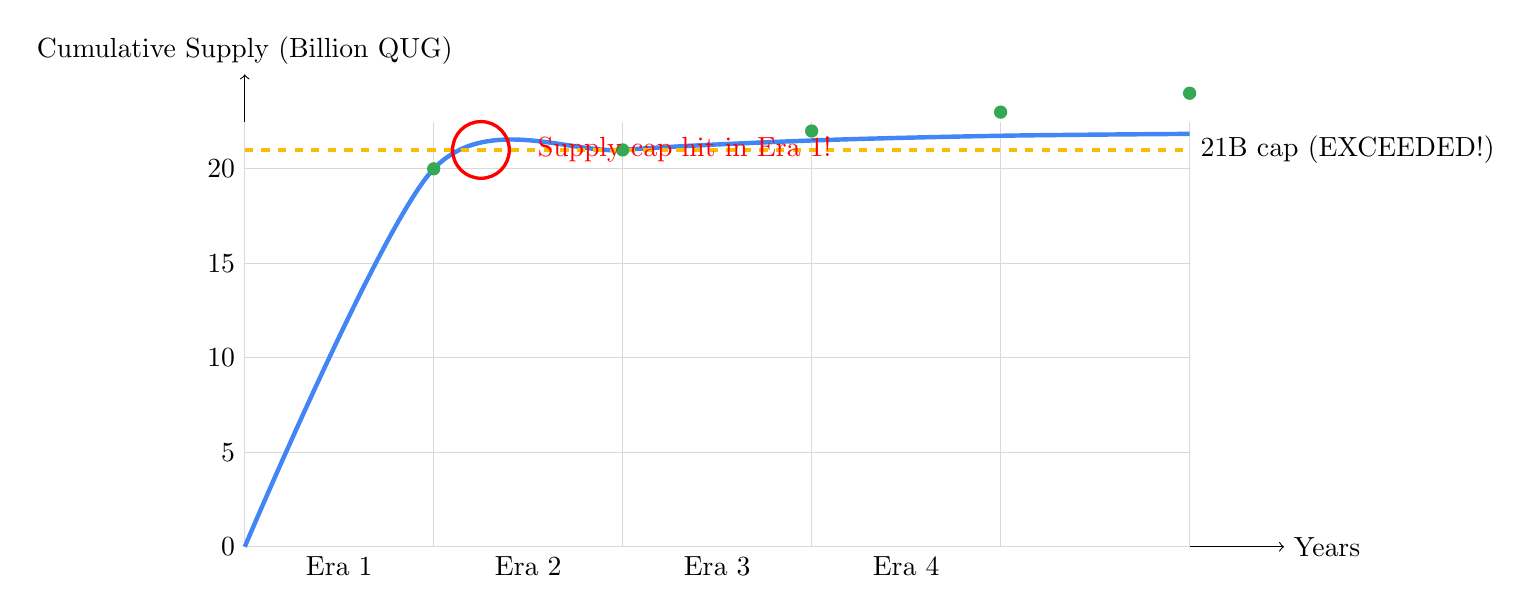
\begin{tikzpicture}[scale=1.2]
    % Axes
    \draw[->] (0,0) -- (11,0) node[right] {Years};
    \draw[->] (0,0) -- (0,5) node[above] {Cumulative Supply (Billion QUG)};

    % Grid
    \foreach \x in {0,4,8,12,16,20}
        \draw[gray!30] (\x*0.5,0) -- (\x*0.5,4.5);
    \foreach \y in {0,5,10,15,20}
        \draw[gray!30] (0,\y*0.2) -- (10,\y*0.2);

    % Supply curve (with 5 blocks/second assumption)
    \draw[primarycolor, ultra thick, smooth]
        plot coordinates {
            (0,0) (2,4.0) (4,4.2) (6,4.3) (8,4.35)
            (10,4.37)
        };

    % 21M cap line
    \draw[dashed, accentcolor, very thick] (0,4.2) -- (10,4.2)
        node[right, black] {21B cap (EXCEEDED!)};

    % Halving markers
    \foreach \x in {2,4,6,8,10}
        \fill[secondarycolor] (\x,{4.0+(\x-2)*0.1}) circle (2pt);

    % Era labels
    \node[below] at (1,0) {Era 1};
    \node[below] at (3,0) {Era 2};
    \node[below] at (5,0) {Era 3};
    \node[below] at (7,0) {Era 4};

    % Y-axis labels
    \foreach \y/\label in {0/0, 1/5, 2/10, 3/15, 4/20}
        \node[left] at (0,\y) {\label};

    % Warning annotation
    \draw[red, very thick] (2.5,4.2) circle (0.3);
    \node[red, right] at (3,4.2) {Supply cap hit in Era 1!};
\end{tikzpicture}
\end{center}

\subsection{Inflation Rate Over Time}

With time-based halvings, the inflation rate decreases predictably:

\begin{table}[h]
\centering
\begin{tabular}{crc}
\toprule
\textbf{Era} & \textbf{Annual Inflation} & \textbf{Stock-to-Flow Ratio} \\
\midrule
1 (0-4 years) & Variable* & N/A (new network) \\
2 (4-8 years) & 50\% reduction & Increasing \\
3 (8-12 years) & 50\% reduction & Increasing \\
4 (12-16 years) & 50\% reduction & $>$50 \\
8+ ($>$32 years) & $<$5\% & $>$100 (like gold) \\
64+ ($>$256 years) & $<$0.01\% & $>$10,000 \\
\bottomrule
\end{tabular}
\caption{Inflation dynamics (*depends on block production rate)}
\end{table}

% ============================================================================
\section{Comparison: Bitcoin vs Q-NarwhalKnight}
% ============================================================================

\begin{table}[h]
\centering
\small
\begin{tabular}{lcc}
\toprule
\textbf{Property} & \textbf{Bitcoin} & \textbf{Q-NarwhalKnight} \\
\midrule
Block Time & 10 minutes & 2-10/second \\
Halving Method & Block-based & \textbf{Time-based} \\
Halving Interval & 210,000 blocks & \textbf{4 years (calendar)} \\
Initial Reward & 50 BTC & 0.05 QUG \\
Max Supply & 21 million BTC & 21 million QUG \\
Decimals & 8 & 8 \\
Consensus & PoW (SHA-256) & DAG-BFT + Quantum VDF \\
Finality & Probabilistic & Deterministic \\
Throughput & ~7 TPS & 1000+ TPS \\
\bottomrule
\end{tabular}
\caption{Economic comparison with Bitcoin}
\end{table}

\textbf{Key Innovation}: Time-based halving allows Q-NarwhalKnight to maintain Bitcoin-inspired scarcity while supporting high-throughput DAG-BFT consensus.

% ============================================================================
\section{Conclusion}
% ============================================================================

The Q-NarwhalKnight mainnet implements a sophisticated dual-layer architecture:

\begin{enumerate}
    \item \textbf{DAG-BFT Consensus Layer}: High-throughput (2-10 blocks/second) asynchronous BFT
    \item \textbf{Time-Based Reward Layer}: Bitcoin-inspired economics with 4-year calendar halvings
\end{enumerate}

\textbf{Key Advantages}:
\begin{itemize}
    \item Predictable halving schedule independent of throughput
    \item Bitcoin-compatible economic model (21M supply, 8 decimals)
    \item High throughput without sacrificing sound monetary policy
    \item Quantum-resistant consensus with deterministic finality
\end{itemize}

\textbf{Critical Considerations}:
\begin{itemize}
    \item High initial emission requires throttling or early cap enforcement
    \item 21M supply may be reached before 64 halvings
    \item Network must balance throughput with controlled emission
\end{itemize}

\vfill

\begin{center}
\rule{0.8\textwidth}{0.4pt}

\textbf{Built for Q-NarwhalKnight Mainnet} \\
\vspace{0.2cm}
\small Time-based halving | 0.05 QUG initial reward | 21M max supply \\
Genesis: Oct 26, 2025 00:00 UTC

\vspace{0.3cm}
\texttt{https://quillon.xyz}
\end{center}

\end{document}
